\chapter{质子核磁共振}\label{ch:g12:proton-nmr}

在医院里，病人躺在核磁共振扫描仪的圆环之中，
屏幕上便出现人体软组织的图像，该图像由其中水和脂肪里
氢\omterm{def:g9:inside-the-atom:nucleus}{原子核}的响应构成。在化学实验室里，一支装有几毫克化合物的小玻璃管
被放入强磁铁的孔道中，同样的原理也能产生一张谱图：
强磁场、射频信号，以及对此作出响应的氢\omterm{def:g9:inside-the-atom:nucleus}{原子核}。
在化学家的波谱仪中，每个氢\omterm{def:g9:inside-the-atom:nucleus}{原子核}因相邻\omterm{def:g7:atoms-and-molecules:atom}{原子}的不同，
而产生略有差异的响应，
谱图便是\omterm{def:g7:atoms-and-molecules:molecule}{分子}中氢\omterm{def:g7:atoms-and-molecules:atom}{原子}的
一幅“地图”。

\begin{recall}
\omterm{def:g11:infrared:spectrum}{红外光谱}可以显示\omterm{def:g7:atoms-and-molecules:molecule}{分子}含有哪些化学键
（见\cref{ch:g11:infrared}）。\omterm{def:g11:functional-groups:functional-group}{官能团}、同系物与\omterm{def:g11:organic-skeletons:isomer}{同分异构体}
（见\cref{ch:g11:functional-groups}、\cref{ch:g11:organic-skeletons}）。
\end{recall}

\begin{omfigure}
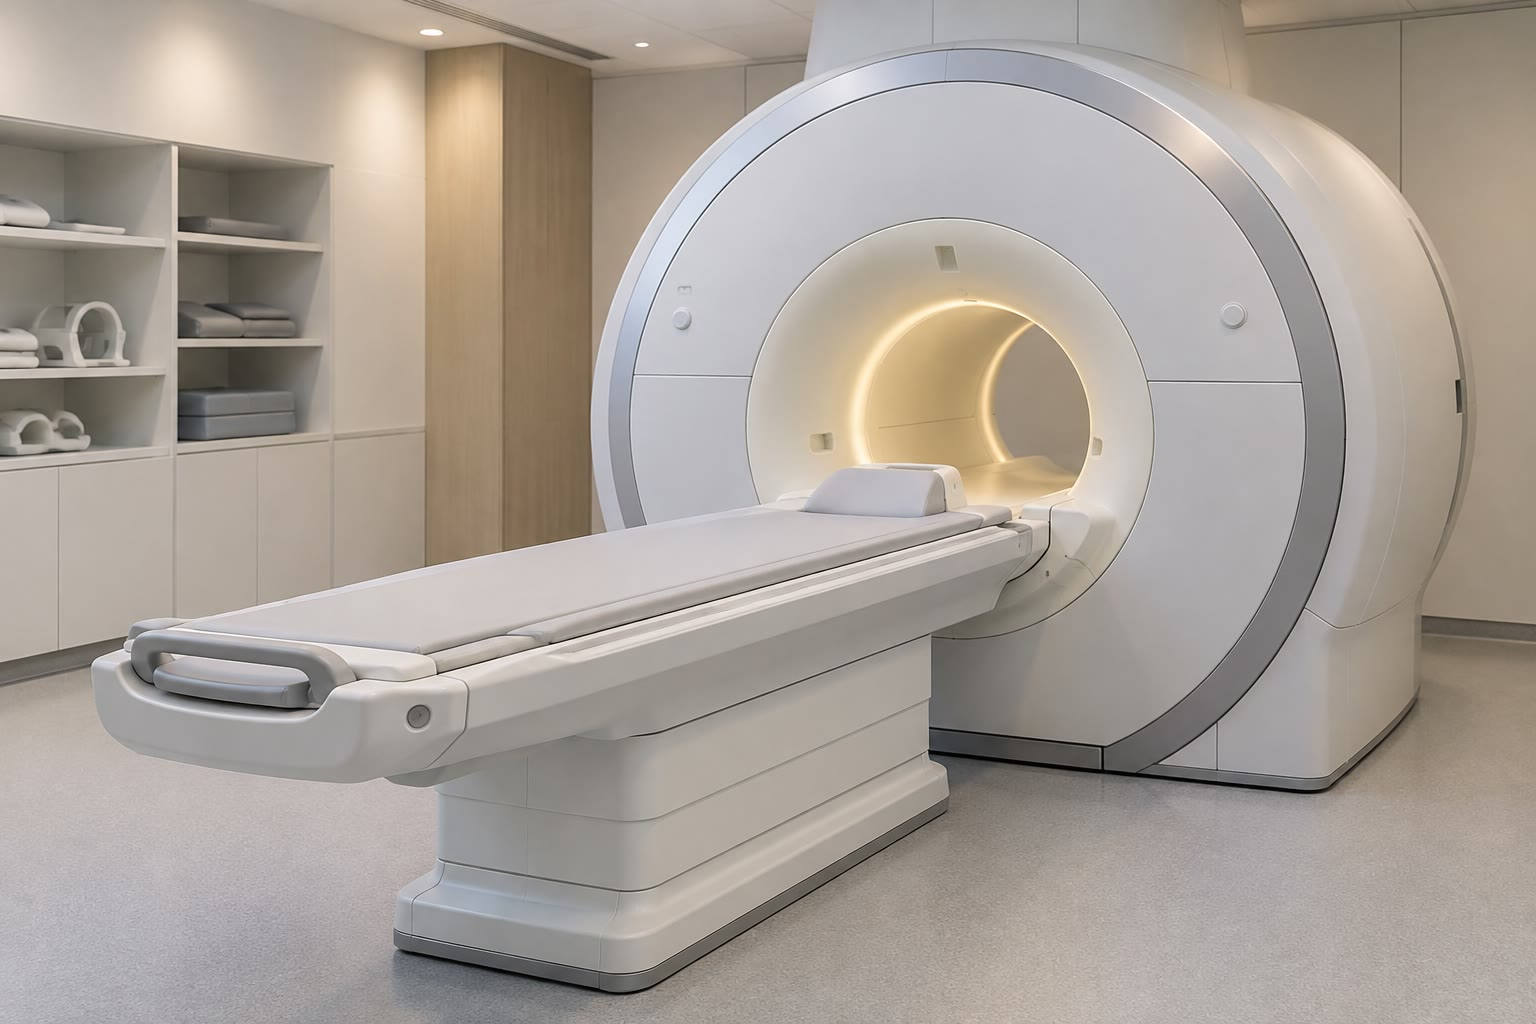
\includegraphics[width=0.48\linewidth]{images/book1/ai/g12-mri-room.jpg}

{\small 核磁共振扫描仪：与化学家的
核磁共振波谱仪遵循相同的物理原理。}
\end{omfigure}

\section{磁场中的质子}

氢\omterm{def:g7:atoms-and-molecules:atom}{原子}的\omterm{def:g9:inside-the-atom:nucleus}{原子核}就是一个\omterm{def:g9:inside-the-atom:proton}{质子}。置于强磁场中时，
它会吸收特定频率的射频波；其中的原理属于物理学范畴，
此处无需说明。对化学家而言，重要的是\omterm{def:g9:inside-the-atom:proton}{质子}周围的\omterm{def:g9:inside-the-atom:nucleus}{电子}
会对其产生轻微屏蔽，而这种屏蔽取决于近邻的\omterm{def:g7:atoms-and-molecules:atom}{原子}：
与吸\omterm{def:g9:inside-the-atom:nucleus}{电子}能力强的氧\omterm{def:g7:atoms-and-molecules:atom}{原子}相邻的\omterm{def:g9:inside-the-atom:proton}{质子}，会把\omterm{def:g9:inside-the-atom:nucleus}{电子}拉离自身，
其吸收频率与烃链中的\omterm{def:g9:inside-the-atom:proton}{质子}略有不同。
这种差异极其微小，
仅为频率的百万分之几，
通常以百万分率表示。

\begin{omfigure}
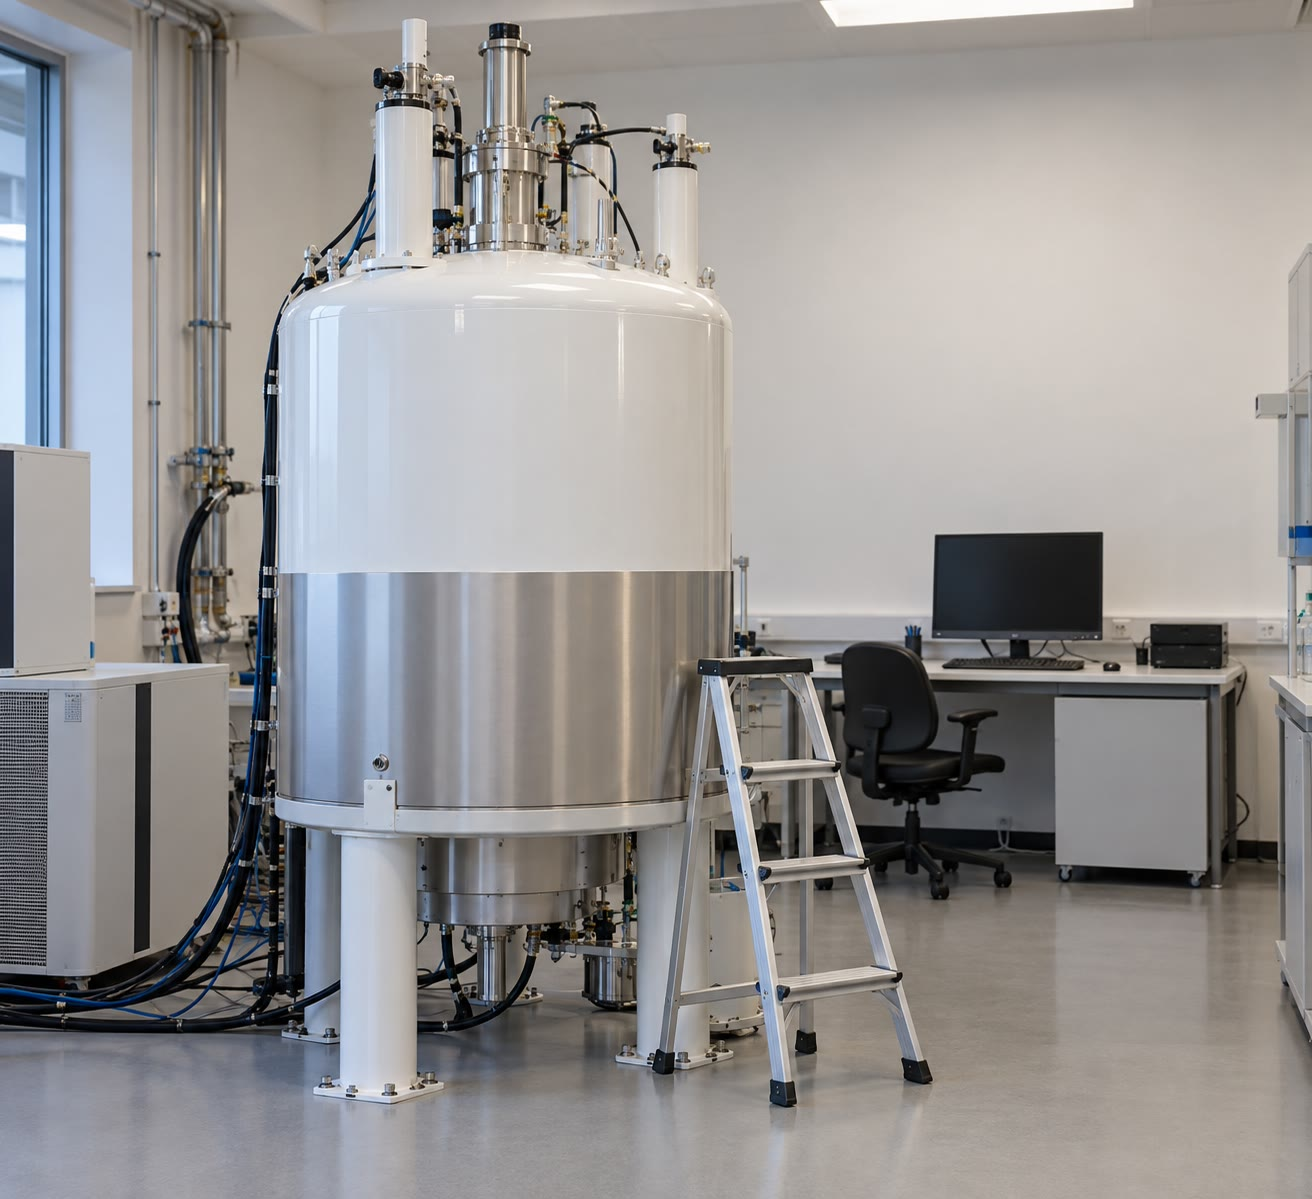
\includegraphics[width=0.42\linewidth]{images/book1/ai/g12-nmr-magnet.jpg}

{\small 核磁共振波谱仪的磁铁。}
\end{omfigure}

\begin{definition}[核磁共振谱，化学位移]\label{def:g12:proton-nmr:spectrum}
\omterm{def:g9:inside-the-atom:proton}{质子}\emph{核磁共振谱}\index{核磁共振谱}表示化合物
中氢\omterm{def:g9:inside-the-atom:nucleus}{原子核}所吸收的信号。信号的位置称为其\emph{化学位移}\index{化学位移}
$\delta$，单位为百万分率（\si{ppm}），
以参照化合物四甲基硅烷\ce{Si(CH3)4}（TMS）的信号为基准，
并定为 $\delta = 0$。
$\delta$ 轴自右向左
递增。
\end{definition}

\begin{proposition}[位移取决于近邻原子]\label{prop:g12:proton-nmr:shift}
% ledger: nmrr:CH3, nmrr:CH2, nmrr:allylic, nmrr:ketone, nmrr:halide, nmrr:alcohol, nmrr:vinylic, nmrr:aryl, nmrr:aldehyde, nmrr:acid
\omterm{def:g9:inside-the-atom:proton}{质子}的\omterm{def:g12:proton-nmr:spectrum}{化学位移}取决于其邻近的\omterm{def:g7:atoms-and-molecules:atom}{原子}：\omterm{def:g9:inside-the-atom:proton}{质子}与吸\omterm{def:g9:inside-the-atom:nucleus}{电子}\omterm{def:g7:atoms-and-molecules:atom}{原子}
或\omterm{def:g10:lewis-and-shape:multiple-bond}{双键}的距离越近，其\omterm{def:g12:proton-nmr:spectrum}{化学位移}越大。常见范围如下
（单位为\si{ppm}）：
\begin{center}
\small
\begin{tabular}{ll@{\qquad}ll}
\hline
化学环境 & $\delta$ & 化学环境 & $\delta$ \\
\hline
链中的 \ce{CH3} & 0.7--1.3 & \ce{H-C-O}（醇、醚、酯） & 3.3--4.5 \\
链中的 \ce{CH2} & 1.2--1.6 & \ce{H-C=C} & 4.5--6.5 \\
\ce{H-C-C=C} & 1.6--2.2 & 苯环上的 H & 6.5--8.0 \\
\ce{H-C-C=O} & 2.0--2.4 & 醛基 \ce{-CHO} & 9.7--10.0 \\
\ce{H-C-X}（\omterm{def:g10:electron-shells:family}{卤素}） & 2.5--4.0 & 羧基 \ce{-COOH} & 11.0--12.0 \\
\hline
\end{tabular}
\end{center}
\end{proposition}

\begin{proof}
由大量化合物的测量结果得出。吸\omterm{def:g9:inside-the-atom:nucleus}{电子}的近邻\omterm{def:g7:atoms-and-molecules:atom}{原子}
把\omterm{def:g9:inside-the-atom:nucleus}{电子}拉离\omterm{def:g9:inside-the-atom:proton}{质子}，使\omterm{def:g9:inside-the-atom:proton}{质子}屏蔽减弱，吸收位置
移向更大的\omterm{def:g12:proton-nmr:spectrum}{化学位移}。
\end{proof}

\begin{omfigure}
\begin{tikzpicture}[font=\small, x=0.75cm, y=0.5cm]
  % delta axis reversed: x = 12 - delta
  \draw[->] (0,0) -- (12.4,0) node[right] {};
  \foreach \d in {12,11,10,9,8,7,6,5,4,3,2,1,0}
    \draw ({12-\d},0) -- ({12-\d},-0.2) node[below, font=\footnotesize] {\d};
  \node[below=14pt] at (6,-0.3) {$\delta$ (\si{ppm})};
  \foreach \a/\b/\y/\c/\l in {
      11.0/12.0/1/omThm/{\ce{COOH}},
      9.7/10.0/2/omThm/{\ce{CHO}},
      6.5/8.0/1/black!60/{苯环},
      4.5/6.5/2/omMeth/{\ce{C=C-H}},
      3.3/4.5/3/omDef/{\ce{H-C-O}},
      2.0/2.4/4/omProp/{\ce{H-C-C=O}},
      0.7/1.6/5/black!45/{链上的 \ce{CH3}、\ce{CH2}}} {
    \fill[\c, rounded corners=1pt] ({12-\b},{\y-0.3}) rectangle ({12-\a},{\y+0.3});
    \node[anchor=west, font=\footnotesize] at ({12-\a+0.1},\y) {\l};
  }
  \draw[thick] (12,0) -- (12,0.6) node[above, font=\footnotesize] {TMS};
\end{tikzpicture}

{\small 按化学环境列出\omterm{def:g9:inside-the-atom:proton}{质子}的吸收位置。靠近氧\omterm{def:g7:atoms-and-molecules:atom}{原子}、
\omterm{def:g10:lewis-and-shape:multiple-bond}{双键}或羧基的\omterm{def:g9:inside-the-atom:proton}{质子}出现在谱图左侧。}
\end{omfigure}

\begin{inthelab}[制备核磁管]
将几毫克化合物溶于约
\qty{0.6}{mL} 的\omterm{def:g6:solutions-and-solubility:solute}{溶剂}中，该\omterm{def:g6:solutions-and-solubility:solute}{溶剂}的氢\omterm{def:g7:atoms-and-molecules:atom}{原子}已被
氘取代（\ce{CDCl3}，氘代氯仿），该\omterm{def:g6:solutions-and-solubility:solute}{溶剂}不产生信号；加入
微量 TMS 作为参照。溶液经\omterm{def:g3:separating-mixtures:filter}{过滤}后装入细玻璃管中，
封盖、贴标签后放入磁铁中。
\end{inthelab}

\section{等效质子}

\begin{definition}[等效质子]\label{def:g12:proton-nmr:equivalent}
若\omterm{def:g9:inside-the-atom:proton}{质子}在\omterm{def:g7:atoms-and-molecules:molecule}{分子}中处于相同的化学环境，则称它们为\emph{等效质子}\index{等效质子}，
因而在相同位移处吸收，
每组等效\omterm{def:g9:inside-the-atom:proton}{质子}给出一个信号。
同一 \ce{CH3} 组中的三个\omterm{def:g9:inside-the-atom:proton}{质子}总是等效的。
\end{definition}

\begin{example}[计数基团]\label{ex:g12:proton-nmr:groups}
丙酮 \ce{CH3-CO-CH3} 含六个\omterm{def:g9:inside-the-atom:proton}{质子}，但只有一组：两个
\ce{CH3} 等同，分居 \ce{C=O} 两侧。
乙醇，\ce{CH3-CH2-OH} 含三组（\ce{CH3}、\ce{CH2}、\ce{OH}），而
乙酸乙酯 \ce{CH3-CO-O-CH2-CH3} 也有三组：其中 \ce{CH3}
与 \ce{C=O} 相邻，\ce{CH2} 与 \ce{O} 相邻，以及
末端的 \ce{CH3}。
\end{example}

\section{积分}

\begin{definition}[积分曲线]\label{def:g12:proton-nmr:integration}
\omterm{def:g12:proton-nmr:spectrum}{核磁共振谱}的\emph{积分曲线}\index{积分曲线}
是画在信号上方的一条曲线，在每个信号处升高一个台阶：
每个台阶的高度与给出该信号的
\omterm{def:g9:inside-the-atom:proton}{质子}数成正比。
\end{definition}

\begin{example}[读取台阶]\label{ex:g12:proton-nmr:steps}
在乙醇的谱图中，三个信号上方的台阶从左到右分别为 2、
1 和 3 个单位，依次对应 \ce{CH2}、\ce{OH} 和 \ce{CH3}。只有
比值才有意义：台阶为 12、6 和 18 mm 时，表示的是同一件事。
\end{example}

\section{裂分与 \texorpdfstring{$n+1$}{n+1} 规则}


\begin{definition}[多重峰、$n+1$ 规则]\label{def:g12:proton-nmr:multiplet}
一个信号常被裂分为若干条靠近的谱线：\emph{多重峰}\index{多重峰}
（单峰、双峰、三重峰、四重峰、\dots{}，分别对应 1、2、3、4 条谱线）。由
\emph{$n+1$ 规则}\index{$n+1$ 规则}可知，一组\omterm{def:g12:proton-nmr:equivalent}{等效质子}，
其相邻碳\omterm{def:g7:atoms-and-molecules:atom}{原子}上共带有 $n$ 个与之不等效的\omterm{def:g9:inside-the-atom:proton}{质子}，
则该组\omterm{def:g9:inside-the-atom:proton}{质子}给出 $n+1$ 条谱线，其强度比
遵循帕斯卡三角形。
\end{definition}

\begin{proposition}[相邻质子引起的裂分]\label{prop:g12:proton-nmr:n-plus-one}
在\omterm{def:g7:atoms-and-molecules:molecule}{分子} \ce{CH3-CH2-X}（X 中不含氢）中，\ce{CH3} 的信号
为三重峰（相邻 2 个\omterm{def:g9:inside-the-atom:proton}{质子}），\ce{CH2} 的信号为四重峰
（相邻 3 个\omterm{def:g9:inside-the-atom:proton}{质子}）。与氧\omterm{def:g7:atoms-and-molecules:atom}{原子}或氮\omterm{def:g7:atoms-and-molecules:atom}{原子}相连的\omterm{def:g9:inside-the-atom:proton}{质子}
通常给出单峰，且不使相邻\omterm{def:g9:inside-the-atom:proton}{质子}发生裂分。
\end{proposition}

\begin{proof}
在本阶段不加证明地承认：每个相邻\omterm{def:g9:inside-the-atom:proton}{质子}依其自身状态使信号略微向高场或低场移动，
各种组合给出 $n+1$ 条谱线；
其物理原理见本科一年级分册。与 O 或 N 相连的\omterm{def:g9:inside-the-atom:proton}{质子}
在\omterm{def:g7:atoms-and-molecules:molecule}{分子}之间快速交换，从而平均掉了它们的影响。
\end{proof}

\begin{omfigure}
\begin{tikzpicture}[font=\small]
  % Pascal's triangle
  \foreach \r/\vals in {0/{1}, 1/{1,1}, 2/{1,2,1}, 3/{1,3,3,1}, 4/{1,4,6,4,1}} {
    \foreach \v [count=\i from 0] in \vals
      \node at ({\i*0.7 - \r*0.35}, {-\r*0.55}) {\v};
    \node[anchor=east, font=\footnotesize, black!60] at (-2.0,{-\r*0.55}) {$n = \r$};
  }
  % multiplets
  \begin{scope}[xshift=4.2cm, yshift=-2.4cm]
    \foreach \x/\name/\hs in {0/单峰/{1}, 1.4/二重峰/{1,1}, 3.0/三重峰/{1,2,1},
                              4.9/四重峰/{1,3,3,1}} {
      \foreach \h [count=\i from 0] in \hs {
        \draw[very thick, omDef] ({\x + \i*0.22},0) -- ({\x + \i*0.22},{\h*0.55});
      }
      \node[anchor=north, font=\footnotesize] at ({\x+0.3},-0.1) {\name};
    }
  \end{scope}
\end{tikzpicture}

{\small 帕斯卡三角形给出 $n+1$ 条谱线的相对强度，这些谱线
来自被 $n$ 个相邻\omterm{def:g9:inside-the-atom:proton}{质子}裂分的信号：1:1、1:2:1、1:3:3:1。}
\end{omfigure}

\begin{omfigure}
\newcommand{\nmrpanel}[4]{% file part, title, xmax, ymax
\begin{tikzpicture}
\begin{axis}[width=\linewidth, height=4.2cm, x dir=reverse, xmin=0,
    xmax=#3, ymin=0, ymax=#4, ytick=\empty, axis y line=none,
    axis x line*=bottom, xlabel={化学位移 $\delta$ (\si{ppm})},
    tick label style={font=\scriptsize}, label style={font=\scriptsize},
    title={\small #2}, title style={yshift=-3pt}]
  \addplot[omDef, thin] table[x=delta, y=I] {figdata/out/grade-12-proton-nmr-#1.dat};
  \addplot[omProp, thick] table[x=delta, y expr=0.15+\thisrow{integral}*0.11]
    {figdata/out/grade-12-proton-nmr-#1.dat};
\end{axis}
\end{tikzpicture}}
\begin{minipage}{0.49\linewidth}\nmrpanel{a}{A: 乙醇}{5}{1.15}\end{minipage}\hfill
\begin{minipage}{0.49\linewidth}\nmrpanel{b}{B: 乙酸乙酯}{5}{1.15}\end{minipage}

\begin{minipage}{0.49\linewidth}\nmrpanel{c}{C: 丙酮}{5}{1.15}\end{minipage}\hfill
\begin{minipage}{0.49\linewidth}\nmrpanel{e}{D: 乙酸甲酯}{5}{1.15}\end{minipage}

\begin{minipage}{\linewidth}\nmrpanel{d}{E: 丙酸}{12.5}{1.15}\end{minipage}

{\small \omterm{def:g9:inside-the-atom:proton}{质子}\omterm{def:g12:proton-nmr:spectrum}{核磁共振谱}（蓝色）及其\omterm{def:g12:proton-nmr:integration}{积分曲线}
（橙色；每个台阶的高度与其下方信号的
\omterm{def:g9:inside-the-atom:proton}{质子}数成正比）。\omterm{def:g12:proton-nmr:spectrum}{化学位移}取自 \ce{CDCl3} 中实测的谱图；
谱线形状与间距由简化模型绘制。}
\end{omfigure}

\begin{example}[读谱图]\label{ex:g12:proton-nmr:reading}
% ledger: nmr:ethylethanoate-OCH2, nmr:ethylethanoate-COCH3, nmr:ethylethanoate-CH3, nmr:ethanol-CH2, nmr:ethanol-CH3, nmr:ethanol-OH, nmr:acetone, nmr:propanoic-CH2, nmr:propanoic-CH3, nmr:propanoic-OH, nmr:meoac-OCH3, nmr:meoac-COCH3
乙酸乙酯（B）给出一组四重峰，含 2 个\omterm{def:g9:inside-the-atom:proton}{质子}，位于 \qty{4.12}{ppm}
（\ce{O-CH2}，与氧及一个 \ce{CH3} 相邻）；一组单峰，含 3 个\omterm{def:g9:inside-the-atom:proton}{质子}，位于
\qty{2.04}{ppm}（\ce{CH3-C=O}，无相邻\omterm{def:g9:inside-the-atom:proton}{质子}）；一组三重峰，含 3 个
\omterm{def:g9:inside-the-atom:proton}{质子}，位于 \qty{1.26}{ppm}（\ce{CH3}，与一个 \ce{CH2} 相邻）。丙酮（C）
只给出一个单峰，含 6 个\omterm{def:g9:inside-the-atom:proton}{质子}，位于 \qty{2.16}{ppm}。丙酸（E）
有一组四重峰，位于 \qty{2.39}{ppm}；一组三重峰，位于 \qty{1.16}{ppm}；
最左侧还有一个单峰，位于 \qty{11.7}{ppm}，是其酸性\omterm{def:g9:inside-the-atom:proton}{质子}。
\end{example}

\section{综合运用红外光谱与核磁共振谱}


\begin{method}[根据红外光谱与核磁共振谱鉴定分子]\label{met:g12:proton-nmr:identify}
\begin{enumerate}
  \item 由\omterm{def:g11:organic-skeletons:formulas}{分子式}列出可能的\omterm{def:g11:organic-skeletons:isomer}{同分异构体}及其
        \omterm{def:g11:functional-groups:functional-group}{官能团}。
  \item \omterm{def:g11:infrared:spectrum}{红外光谱}：寻找 \qty{1700}{cm^{-1}} 附近的 \ce{C=O} 吸收峰，以及
        \ce{O-H} 或 \ce{N-H} 的吸收峰；划去不符合的
        \omterm{def:g11:organic-skeletons:isomer}{同分异构体}。
  \item \omterm{def:g12:proton-nmr:spectrum}{核磁共振谱}：数出信号数（即\omterm{def:g12:proton-nmr:equivalent}{等效质子}组数），读出
        积分（每组\omterm{def:g9:inside-the-atom:proton}{质子}数）、峰的多重性（相邻\omterm{def:g9:inside-the-atom:proton}{质子}数）以及
        \omterm{def:g12:proton-nmr:spectrum}{化学位移}（所处化学环境）。
  \item 将各部分拼合为一个结构，并与所有
        观察结果逐一核对。
\end{enumerate}
\end{method}

\begin{example}[两种同分异构体 \ce{C3H6O2}]\label{ex:g12:proton-nmr:isomers}
丙酸 \ce{CH3-CH2-COOH} 与乙酸甲酯 \ce{CH3-CO-O-CH3}
互为\omterm{def:g11:organic-skeletons:isomer}{同分异构体}。\omterm{def:g11:infrared:spectrum}{红外光谱}中，只有丙酸显示很宽的 \ce{O-H}
吸收峰。\omterm{def:g12:proton-nmr:spectrum}{核磁共振谱}（谱图 E 和 D）中，丙酸给出一个三重峰、一个四重峰和
一个位于 \qty{11.7}{ppm} 附近的单峰；酯给出两个单峰，各含 3 个\omterm{def:g9:inside-the-atom:proton}{质子}，
分别位于 3.66（\ce{O-CH3}）和 \qty{2.05}{ppm}（\ce{CH3-C=O}），因为
酯中没有任何带\omterm{def:g9:inside-the-atom:proton}{质子}的碳与另一个带\omterm{def:g9:inside-the-atom:proton}{质子}的碳相邻。
\end{example}

\section{练习}

\begin{exercise}[$\star$]\label{exo:g12:proton-nmr:1}
下列\omterm{def:g7:atoms-and-molecules:molecule}{分子}各含多少组\omterm{def:g12:proton-nmr:equivalent}{等效质子}，从而给出多少个信号：
甲烷；乙烷 \ce{CH3-CH3}；丙烷；甲醇
\ce{CH3-OH}；甲醚 \ce{CH3-O-CH3}？
\end{exercise}

\begin{exercise}[$\star$]\label{exo:g12:proton-nmr:2}
某组\omterm{def:g9:inside-the-atom:proton}{质子}所在碳的相邻碳上有 2 个\omterm{def:g9:inside-the-atom:proton}{质子}，其信号有几条峰，
强度比为多少？对于 3 个和
0 个邻近\omterm{def:g9:inside-the-atom:proton}{质子}的情况，同样回答。
\end{exercise}

\begin{exercise}[$\star$]\label{exo:g12:proton-nmr:3}
某谱图有三个信号，积分台阶高度分别为 15、10 和
15 mm。该\omterm{def:g7:atoms-and-molecules:molecule}{分子}含 8 个\omterm{def:g9:inside-the-atom:proton}{质子}。每个信号分别代表
多少个\omterm{def:g9:inside-the-atom:proton}{质子}？
\end{exercise}

\begin{exercise}[$\star$]\label{exo:g12:proton-nmr:4}
依据\omterm{def:g12:proton-nmr:spectrum}{化学位移}表，醛基\omterm{def:g9:inside-the-atom:proton}{质子}的信号
出现在何处？链中 \ce{CH3} 基团的\omterm{def:g9:inside-the-atom:proton}{质子}又在何处？
\end{exercise}

\begin{exercise}[$\star$]\label{exo:g12:proton-nmr:5}
为何选用 TMS 作参比物，使其\omterm{def:g9:inside-the-atom:proton}{质子}全部等效？
为何\omterm{def:g6:solutions-and-solubility:solute}{溶剂}要用氘代\omterm{def:g7:identifying-substances:characteristic-test}{试剂}？
\end{exercise}

\begin{exercise}[$\star\star$]\label{exo:g12:proton-nmr:6}
预测氯乙烷 \ce{CH3-CH2-Cl} 的谱图：信号数、
积分、峰的多重性及大致\omterm{def:g12:proton-nmr:spectrum}{化学位移}。
\end{exercise}

\begin{exercise}[$\star\star$]\label{exo:g12:proton-nmr:7}
预测 2-丙醇 \ce{(CH3)2CH-OH} 的谱图：特别是 \ce{CH3} 信号和 \ce{CH} 信号的
多重性（假设
\ce{OH} 给出单峰且不发生裂分）。
\end{exercise}

\begin{exercise}[$\star\star$]\label{exo:g12:proton-nmr:8}
三张谱图：(a) 一个单峰；(b) 一个四重峰、一个单峰和一个三重峰，
积分比为 2:3:3；(c) 一个四重峰、一个三重峰和一个位于最左侧的单峰，
积分比为 2:3:1。请将它们分别与乙酸乙酯、丙酮和
丙酸配对。
\end{exercise}

\begin{exercise}[$\star\star$]\label{exo:g12:proton-nmr:9}
利用\omterm{def:g12:proton-nmr:spectrum}{化学位移}图，解释乙酸乙酯中 \ce{CH2}
（\qty{4.12}{ppm}）的峰远比同一乙基中
\ce{CH3}（\qty{1.26}{ppm}）的峰靠左的原因。
\end{exercise}

\begin{exercise}[$\star\star$]\label{exo:g12:proton-nmr:10}
某化合物 \ce{C3H6O} 在
\qty{1715}{cm^{-1}} 处有很强的红外吸收，\omterm{def:g12:proton-nmr:spectrum}{核磁共振谱}仅有一个单峰。试确定其结构，
并说明为何排除丙醛？
\end{exercise}

\begin{exercise}[$\star\star$]\label{exo:g12:proton-nmr:11}
在乙醇的谱图中，为何 \ce{OH} 信号为单峰，且为何
\ce{CH2} 呈现为四重峰，而非更复杂的
信号？
\end{exercise}

\begin{exercise}[$\star\star\star$]\label{exo:g12:proton-nmr:12}
写出四种属于酯或酸的 \ce{C4H8O2} \omterm{def:g11:organic-skeletons:isomer}{同分异构体}的结构
（丁酸、乙酸乙酯、丙酸甲酯、甲酸丙酯，
\dots），并分别预测每种的核磁共振信号数及其
多重性。
\end{exercise}

\begin{exercise}[$\star\star\star$]\label{exo:g12:proton-nmr:13}
将一滴重水 \ce{D2O} 与乙醇溶液\omterm{def:g2:mixing-and-dissolving:mix}{混合}振荡，
再次记录谱图，一个信号消失。是哪一个？为什么？
这对识别 \ce{O-H} \omterm{def:g9:inside-the-atom:proton}{质子}有何帮助？
\end{exercise}

\begin{exercise}[$\star\star\star$]\label{exo:g12:proton-nmr:14}
乙酸乙酯样品中含有少量乙醇。哪些额外信号
会出现在谱图中？若单峰位于
\qty{2.04}{ppm} 处，其积分为 30 mm，小三重峰位于
\qty{1.23}{ppm} 处，积分为 3 mm，估算乙醇与
酯的\omterm{def:g10:the-mole:amount}{物质的量}之比。
\end{exercise}

\begin{exercise}[$\star\star\star$]\label{exo:g12:proton-nmr:15}
2-甲基丙-1-醇为 \ce{(CH3)2CH-CH2-OH}。预测其谱图，
包括各信号、积分以及 \ce{CH3} 与
\ce{CH2} 信号的多重性。哪一个信号的峰数最多？
\end{exercise}

\section{问题：未知溶剂}

\begin{problem}[{周末问题——一瓶仅标有
\ce{C4H8O2} 的\omterm{def:g6:solutions-and-solubility:solute}{溶剂}：它是什么？其\omterm{def:g12:proton-nmr:integration}{积分曲线}
的每一级台阶有多高？}]
\label{pb:g12:proton-nmr:1}
% ledger: nmr:ethylethanoate-OCH2, nmr:ethylethanoate-COCH3, nmr:ethylethanoate-CH3, ir:CO-ester, ir:OH-acid
储藏室里有一瓶\omterm{def:g6:solutions-and-solubility:solute}{溶剂}，标签上只写着“\ce{C4H8O2}”。其
\omterm{def:g11:infrared:spectrum}{红外光谱}在 \qty{1740}{cm^{-1}} 处有一个强吸收带，
在 \qty{3100}{cm^{-1}} 以上则没有吸收带。其\omterm{def:g12:proton-nmr:spectrum}{核磁共振谱}有三个信号：
一个四重峰位于 \qty{4.12}{ppm}，一个单峰位于 \qty{2.04}{ppm}，一个三重峰位于
\qty{1.26}{ppm}。\omterm{def:g12:proton-nmr:integration}{积分曲线}共上升 \qty{72}{mm}。

\medskip
\noindent\textbf{第一部分——候选物质。}
\begin{enumerate}
  \item 检验 \ce{C4H8O2} 是否符合酯或\omterm{def:g11:functional-groups:carboxylic-acid}{羧酸}，且
        其碳链中仅含单键。
  \item 给出丁酸的\omterm{def:g11:organic-skeletons:formulas}{结构简式}与名称，以及三种酯
        乙酸乙酯、丙酸甲酯和甲酸丙酯的\omterm{def:g11:organic-skeletons:formulas}{结构简式}与
        名称。
  \item 它们两两之间共有哪一类\omterm{def:g11:functional-groups:functional-group}{官能团}？
\end{enumerate}

\medskip
\noindent\textbf{第二部分——\omterm{def:g11:infrared:spectrum}{红外光谱}。}
\begin{enumerate}[resume]
  \item \qty{1740}{cm^{-1}} 处的吸收带说明了什么？
  \item 丁酸会出现、而此处缺少的吸收带是什么？
        请将其划掉。
  \item 仅凭\omterm{def:g11:infrared:spectrum}{红外光谱}能否区分三种酯？
\end{enumerate}

\medskip
\noindent\textbf{第三部分——\omterm{def:g12:proton-nmr:spectrum}{核磁共振谱}。}
\begin{enumerate}[resume]
  \item 未知物有几组\omterm{def:g12:proton-nmr:equivalent}{等效质子}？
  \item 四重峰与三重峰合起来说明了什么？
  \item 单峰对其\omterm{def:g9:inside-the-atom:proton}{质子}的相邻基团给出了什么信息？
  \item 四重峰的\omterm{def:g12:proton-nmr:spectrum}{化学位移}为何较大？
  \item 预测丙酸甲酯 \ce{CH3-CH2-CO-O-CH3} 的谱图
        （信号、多重性、近似\omterm{def:g12:proton-nmr:spectrum}{化学位移}）。它是未知物吗？
  \item 预测甲酸丙酯的谱图。它是未知物吗？
\end{enumerate}

\medskip
\noindent\textbf{第四部分——鉴定与积分。}
\begin{enumerate}[resume]
  \item 鉴定未知物，画出其结构，并标注每一组
        信号。
  \item 每个信号对应多少个\omterm{def:g9:inside-the-atom:proton}{质子}？
  \item 8 个\omterm{def:g9:inside-the-atom:proton}{质子}的总积分为 \qty{72}{mm}，
        每个\omterm{def:g9:inside-the-atom:proton}{质子}对应多少毫米？
  \item 计算单峰与三重峰的台阶高度。
  \item 检验三个台阶之和为 \qty{72}{mm}。
  \item 乙酸乙酯闻起来像梨味硬糖，这与
        所确定的化合物类别是否相符？
  \item 给出最终答案：四重峰的积分台阶
        高度是多少？
\end{enumerate}
\end{problem}
